\documentclass{beamer}
\usetheme[
  sectionpage=progressbar,
  numbering=counter,
  titleformat=smallcaps
  % progressbar=frametitle
]{metropolis}             % Use metropolis theme

% Fix needed to make fonts work on ubuntu: https://github.com/matze/mtheme/issues/280
%\setsansfont[	 	  
%    Extension      = .otf,
%    UprightFont    = *-Light,
%    ItalicFont     = *-LightItalic,
%    BoldFont       = *-Regular,
%    BoldItalicFont = *-RegularItalic
%]{FiraSans}
%\setmonofont[
%    Extension   = .otf,
%    UprightFont = *-Regular,
%    BoldFont    = *-Medium
%]{FiraMono}

\usepackage[german]{babel}
\usepackage{xcolor}
\usepackage{hyperref}

\newcommand\ytl[2]{
  \parbox[b]{8em}{\hfill{\color{cyan}\bfseries\sffamily #1}~$\cdots\cdots$~}\makebox[0pt][c]{$\bullet$}\vrule\quad \parbox[c]{4.5cm}{\vspace{7pt}\color{red!40!black!80}\raggedright\sffamily #2.\\[7pt]}\\[-3pt]
}


\definecolor{cioDarkBlue}{HTML}{12254c}
\setbeamercolor{normal text}{%
    fg=cioDarkBlue,
    bg=black!2
}

\graphicspath{{img/}}

\title{Linux Container für den Alltagsgebrauch}
\date{6.4.2019}
\author{Anian Ziegler}
\institute{Augsburger Linux-Infotag}

\begin{document}
  \maketitle

  % % % % % % % % % % % % % % 
  % Was ist ein container?  %
  % % % % % % % % % % % % % %
  \section{Einstieg: Was sind Container?}

  \begin{frame}{Was sind Container?}
    \begin{itemize}[<+->]
      \item Basieren auf Features des Linux Kernels
      \item Isolieren und verpacken Anwendungen
      \item Werden meistens mit Docker verwaltet
      \item \alert{Virtualisierung von Betriebssystem-Features}
    \end{itemize}
  \end{frame}

  \begin{frame}{Was sind Container?}
    \begin{center}
      Container sind keine Hardware-Virtualisierung und kein Emulator.
      Alles passiert in einem einzelnen Kernel.
    \end{center}
  \end{frame}
  
  \begin{frame}{Exkurs: Hardware-Virtualisierung}
    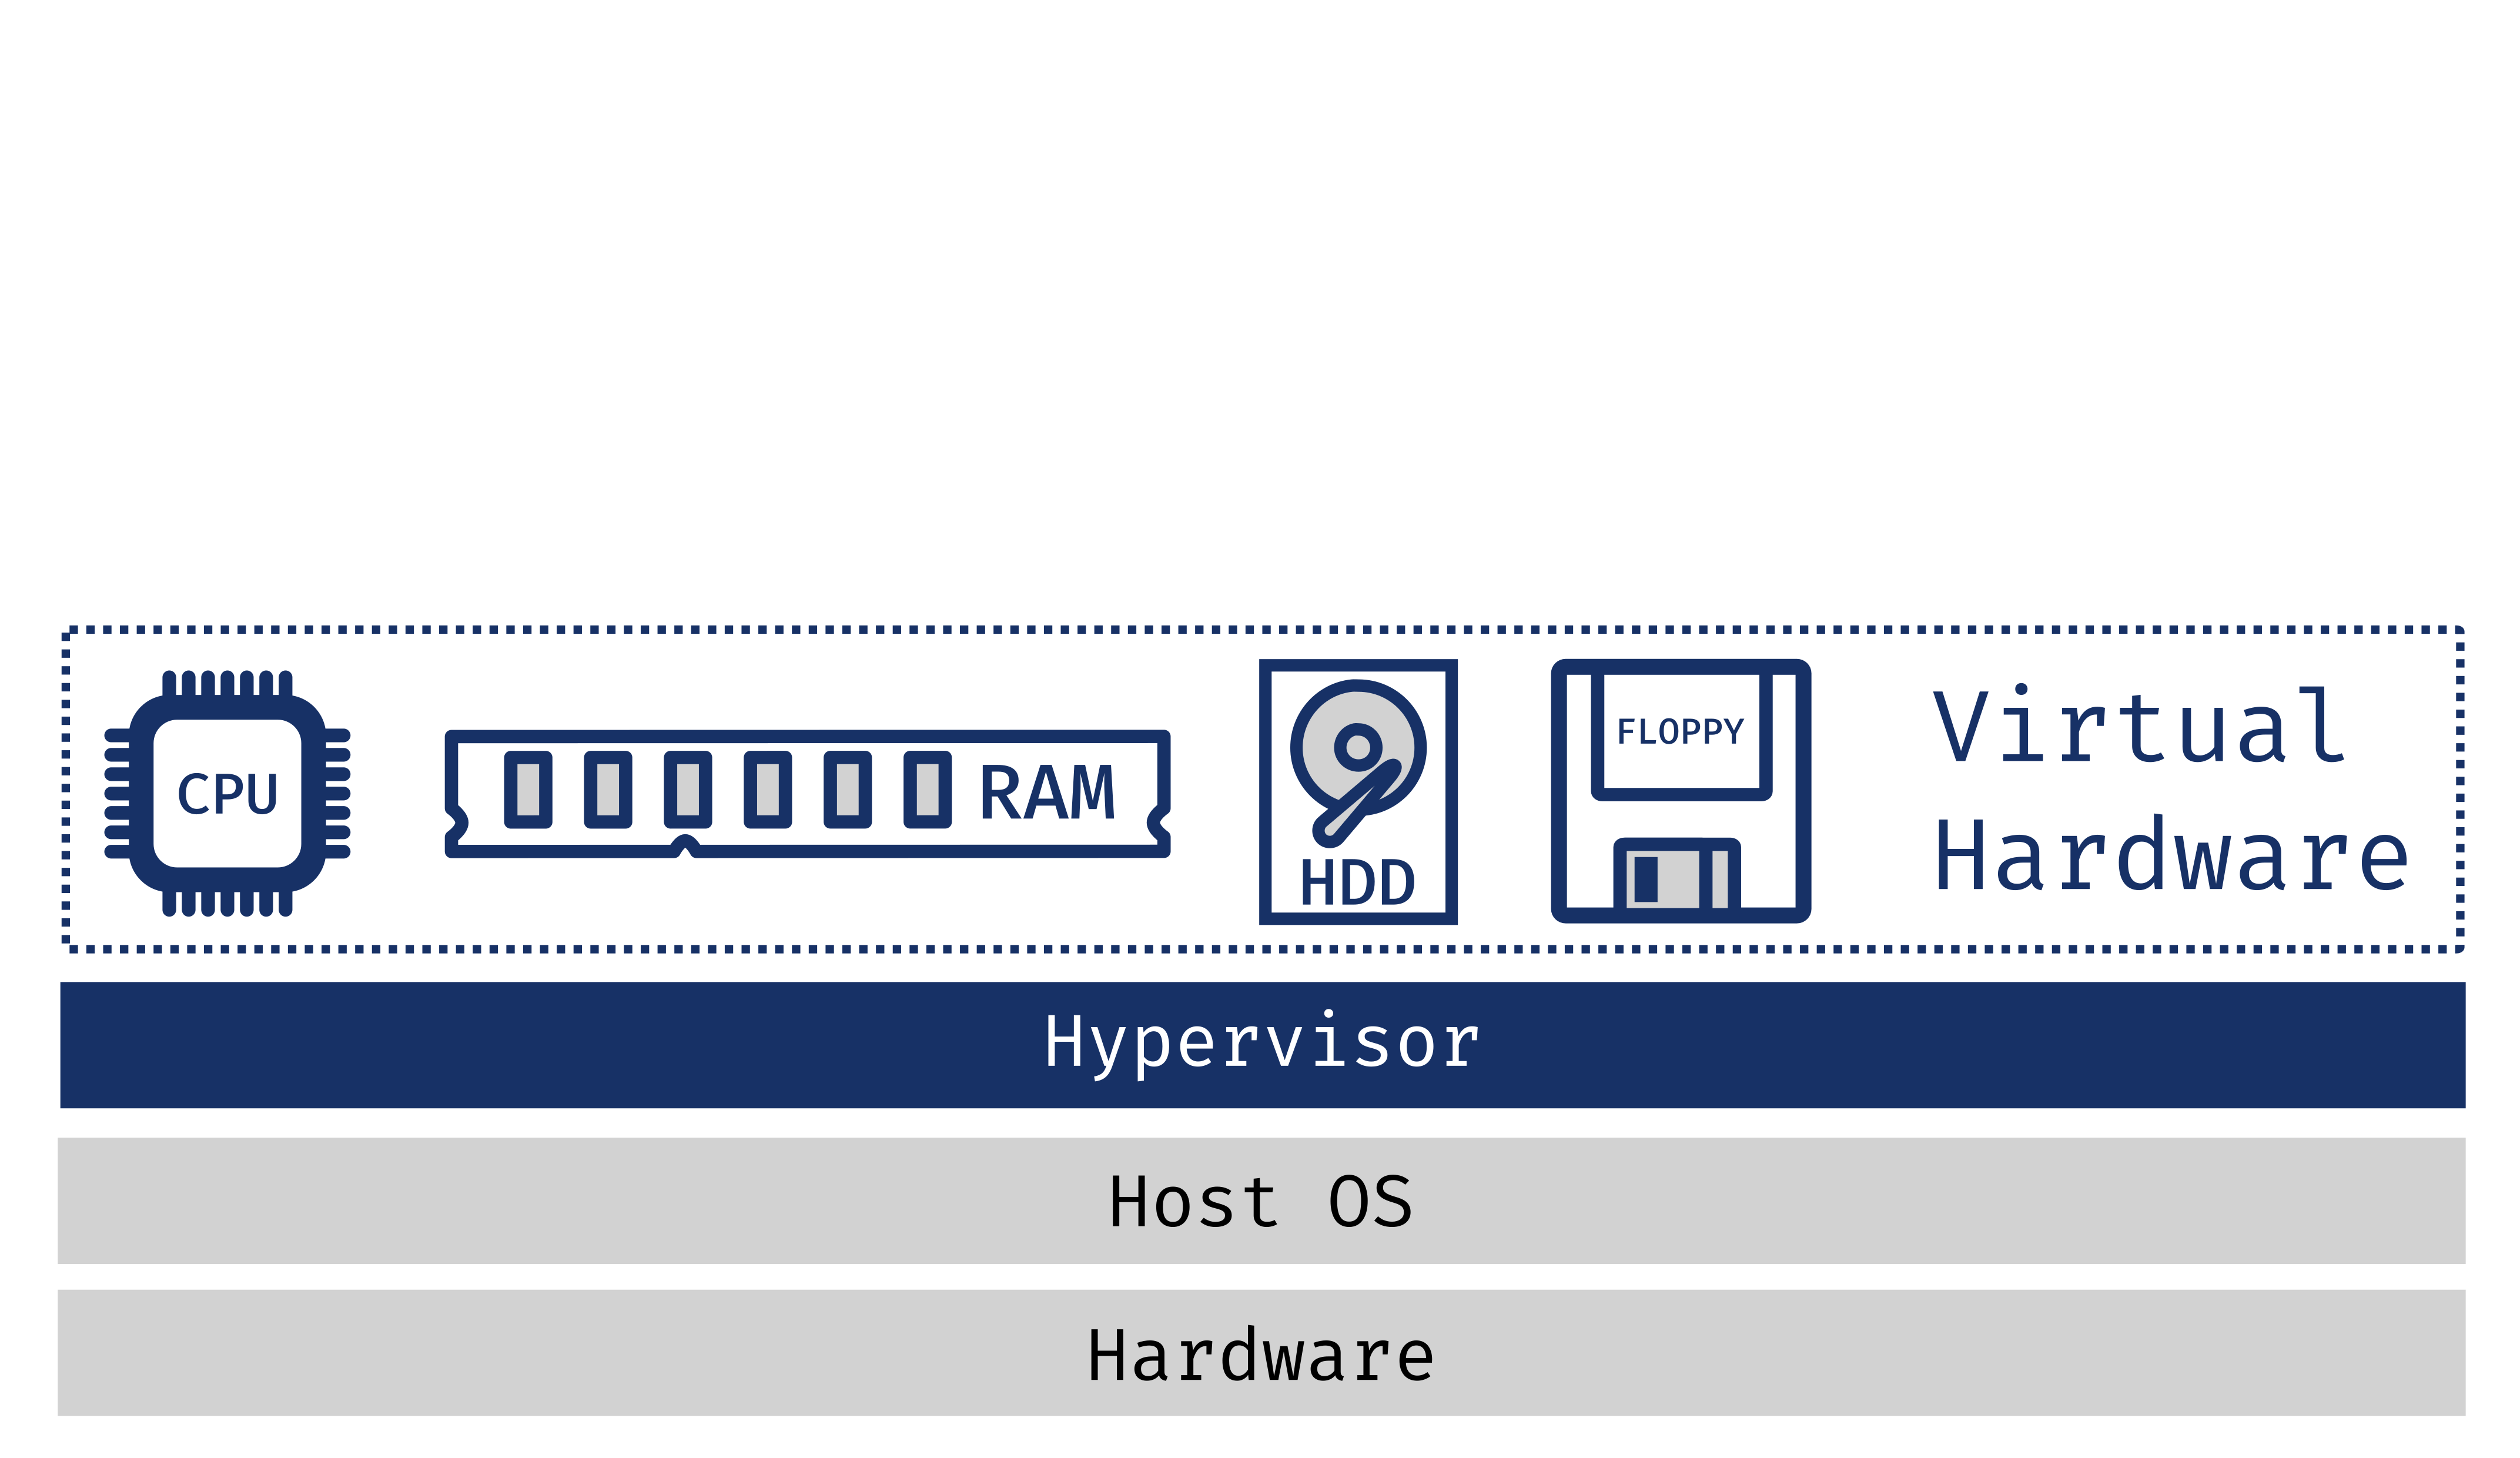
\includegraphics[width=\textwidth]{hypervisor}
  \end{frame}
  \begin{frame}{Exkurs: Hardware-Virtualisierung}
    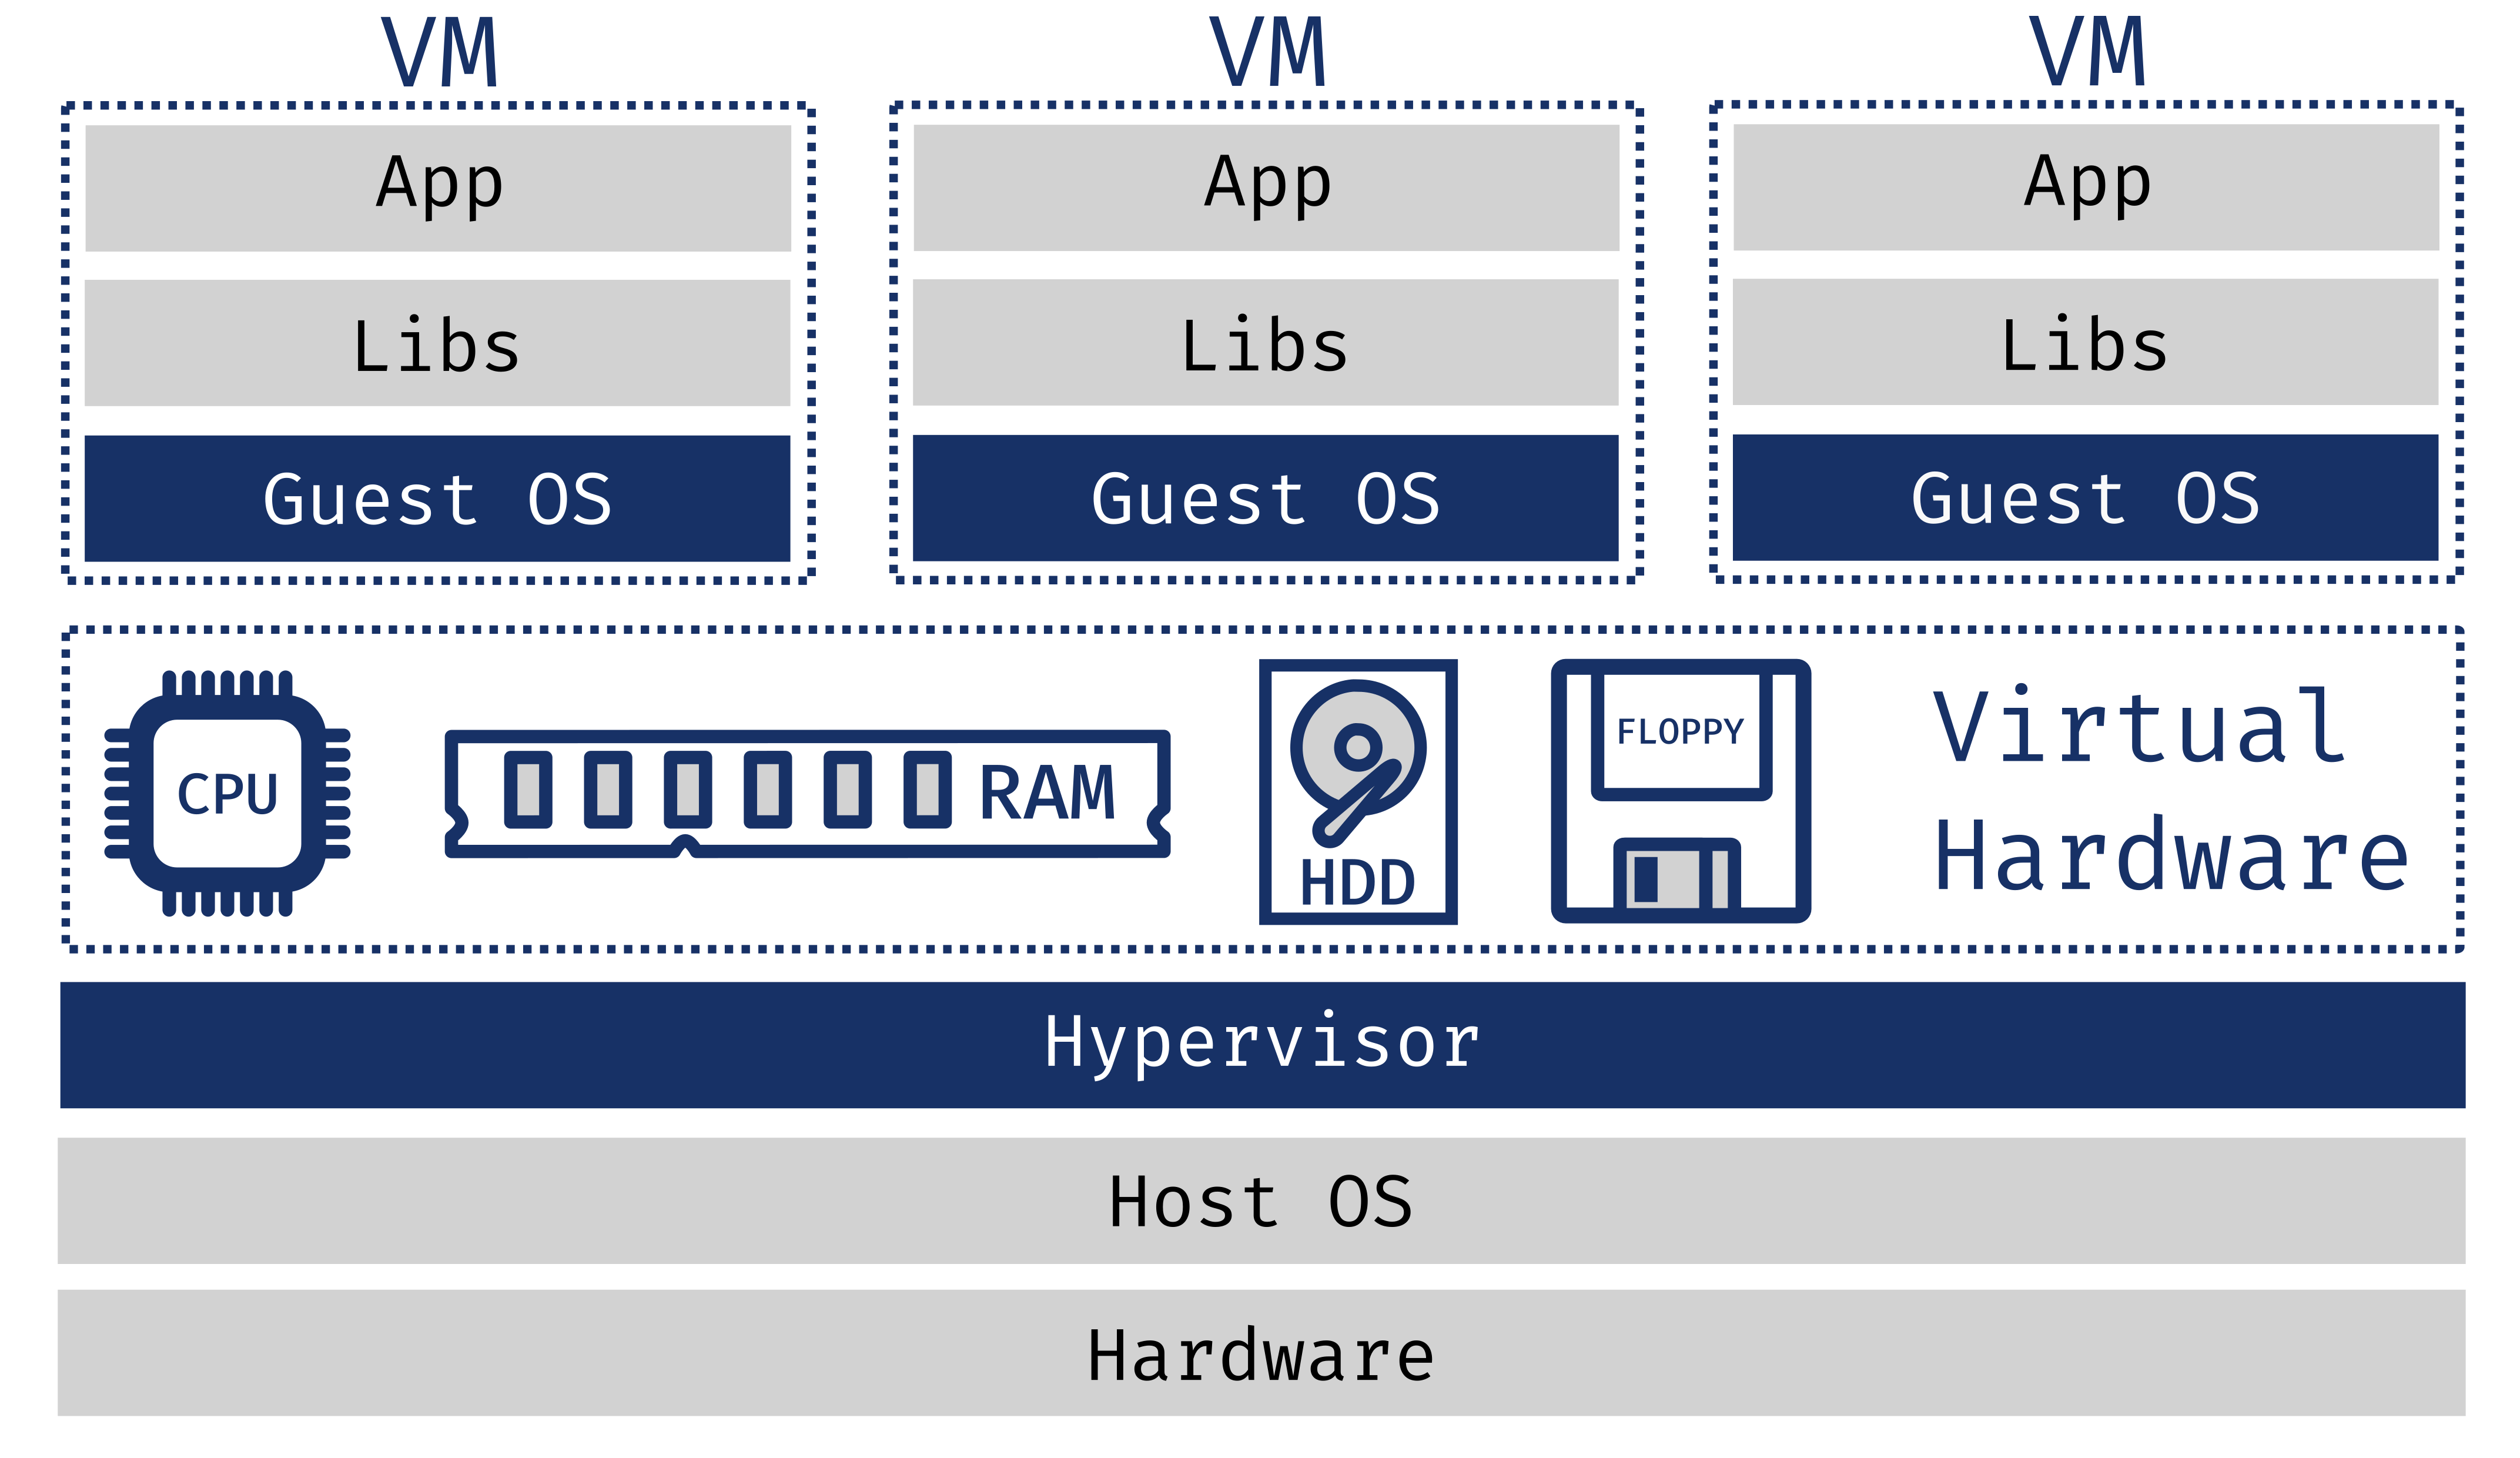
\includegraphics[width=\textwidth]{vms}
  \end{frame}
  
  \begin{frame}{Virtualisierung auf Betriebssystemebene}
    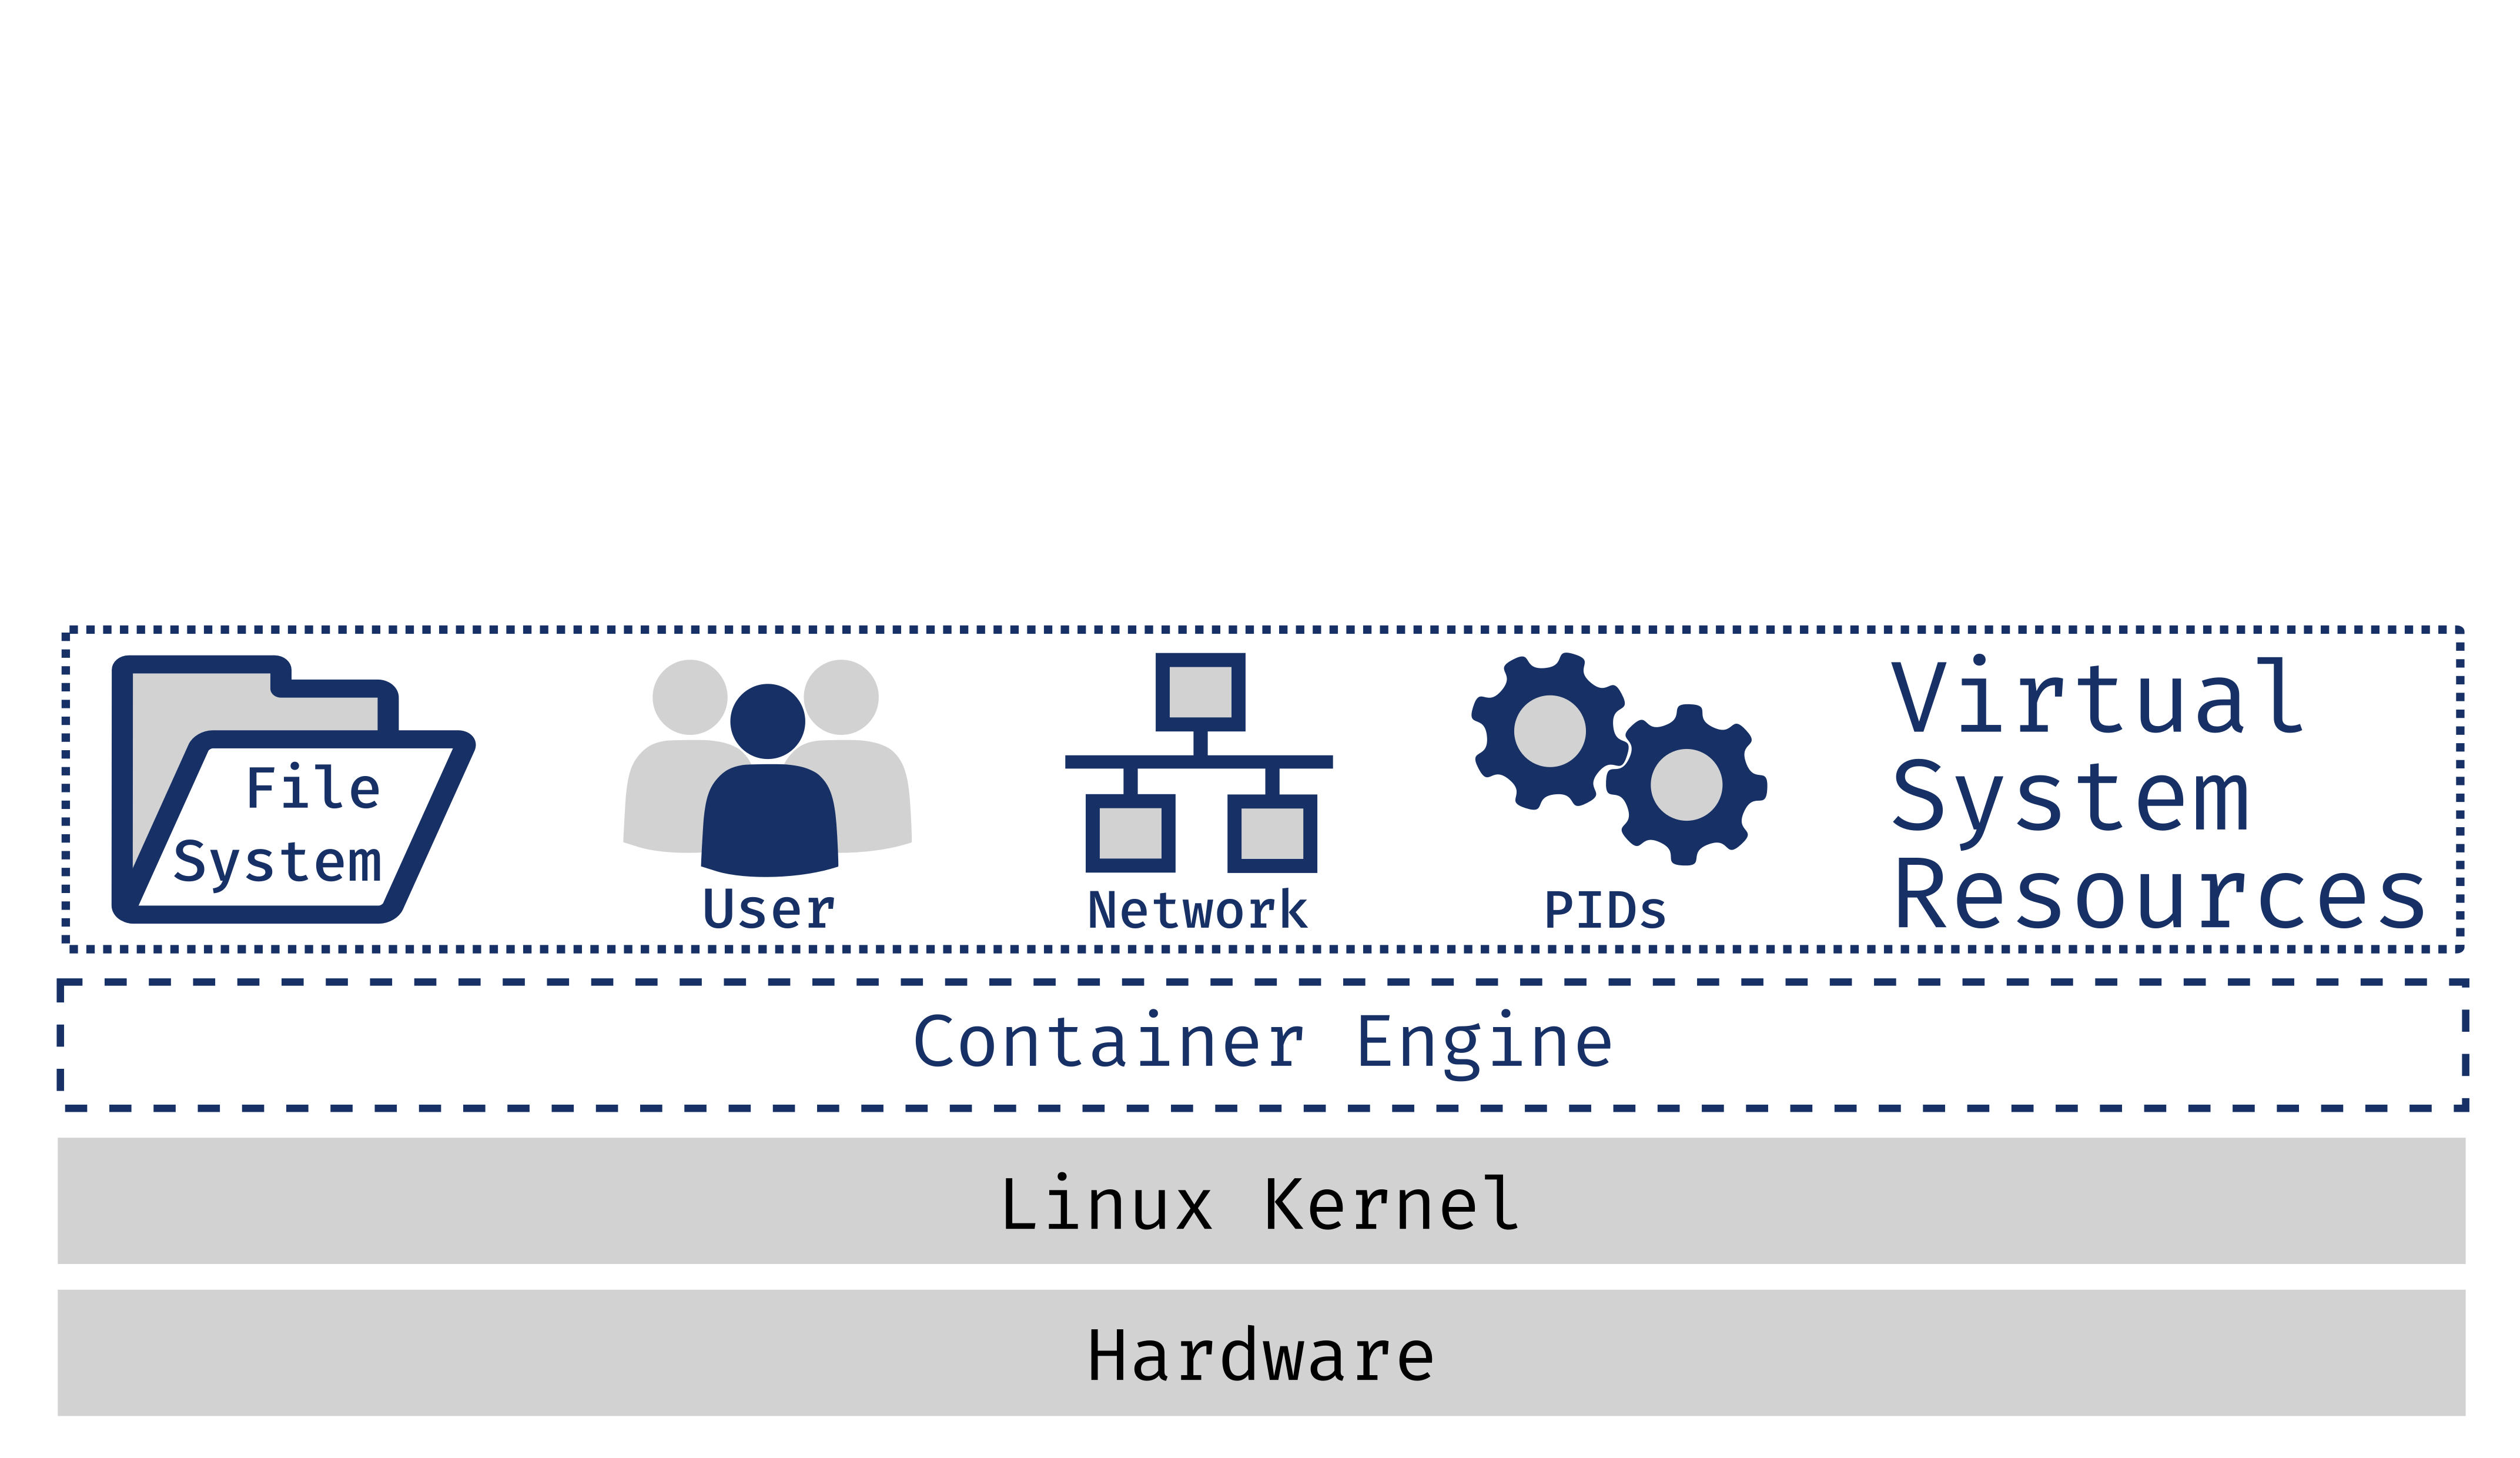
\includegraphics[width=\textwidth]{os-virt}
  \end{frame}
  \begin{frame}{Virtualisierung auf Betriebssystemebene}
    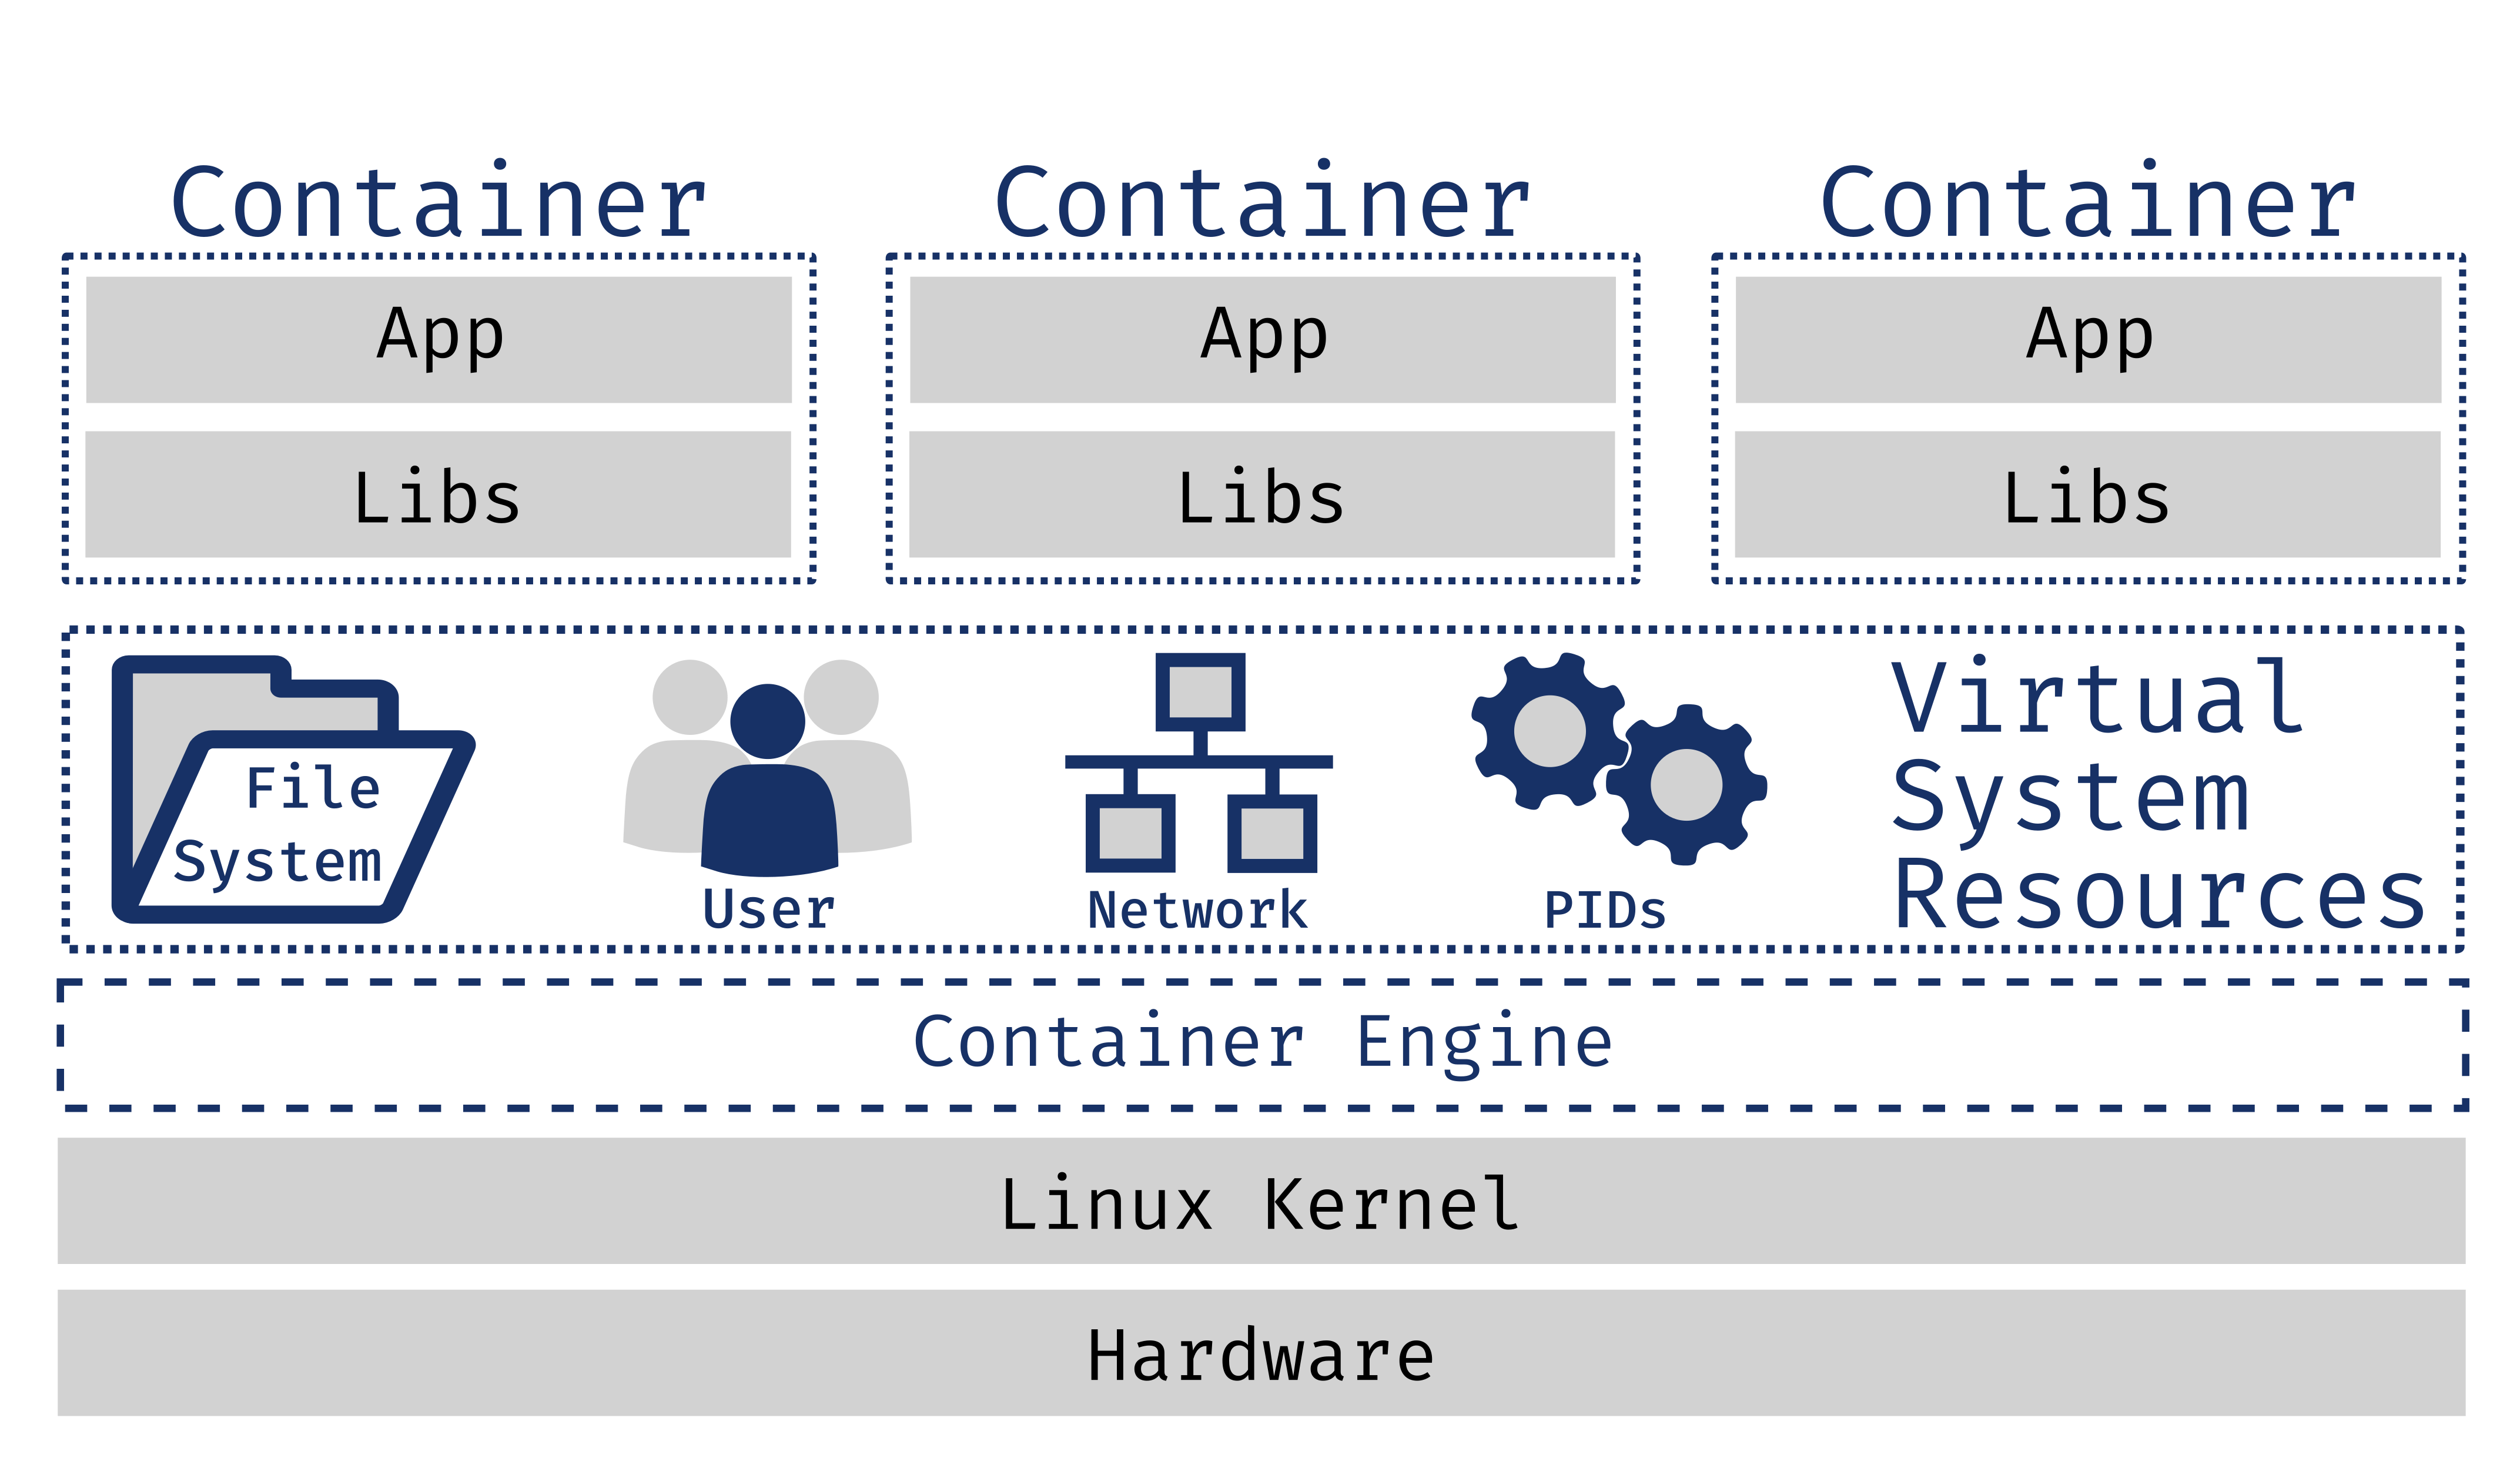
\includegraphics[width=\textwidth]{container}
  \end{frame}

  % % % % % % % % % %
  % Implementierung %
  % % % % % % % % % %
  \section{Implementierung in Linux}

  \begin{frame}{chroot}
    
\includegraphics[width=\textwidth]{fs-tree}
  \end{frame}
  \begin{frame}{chroot}
    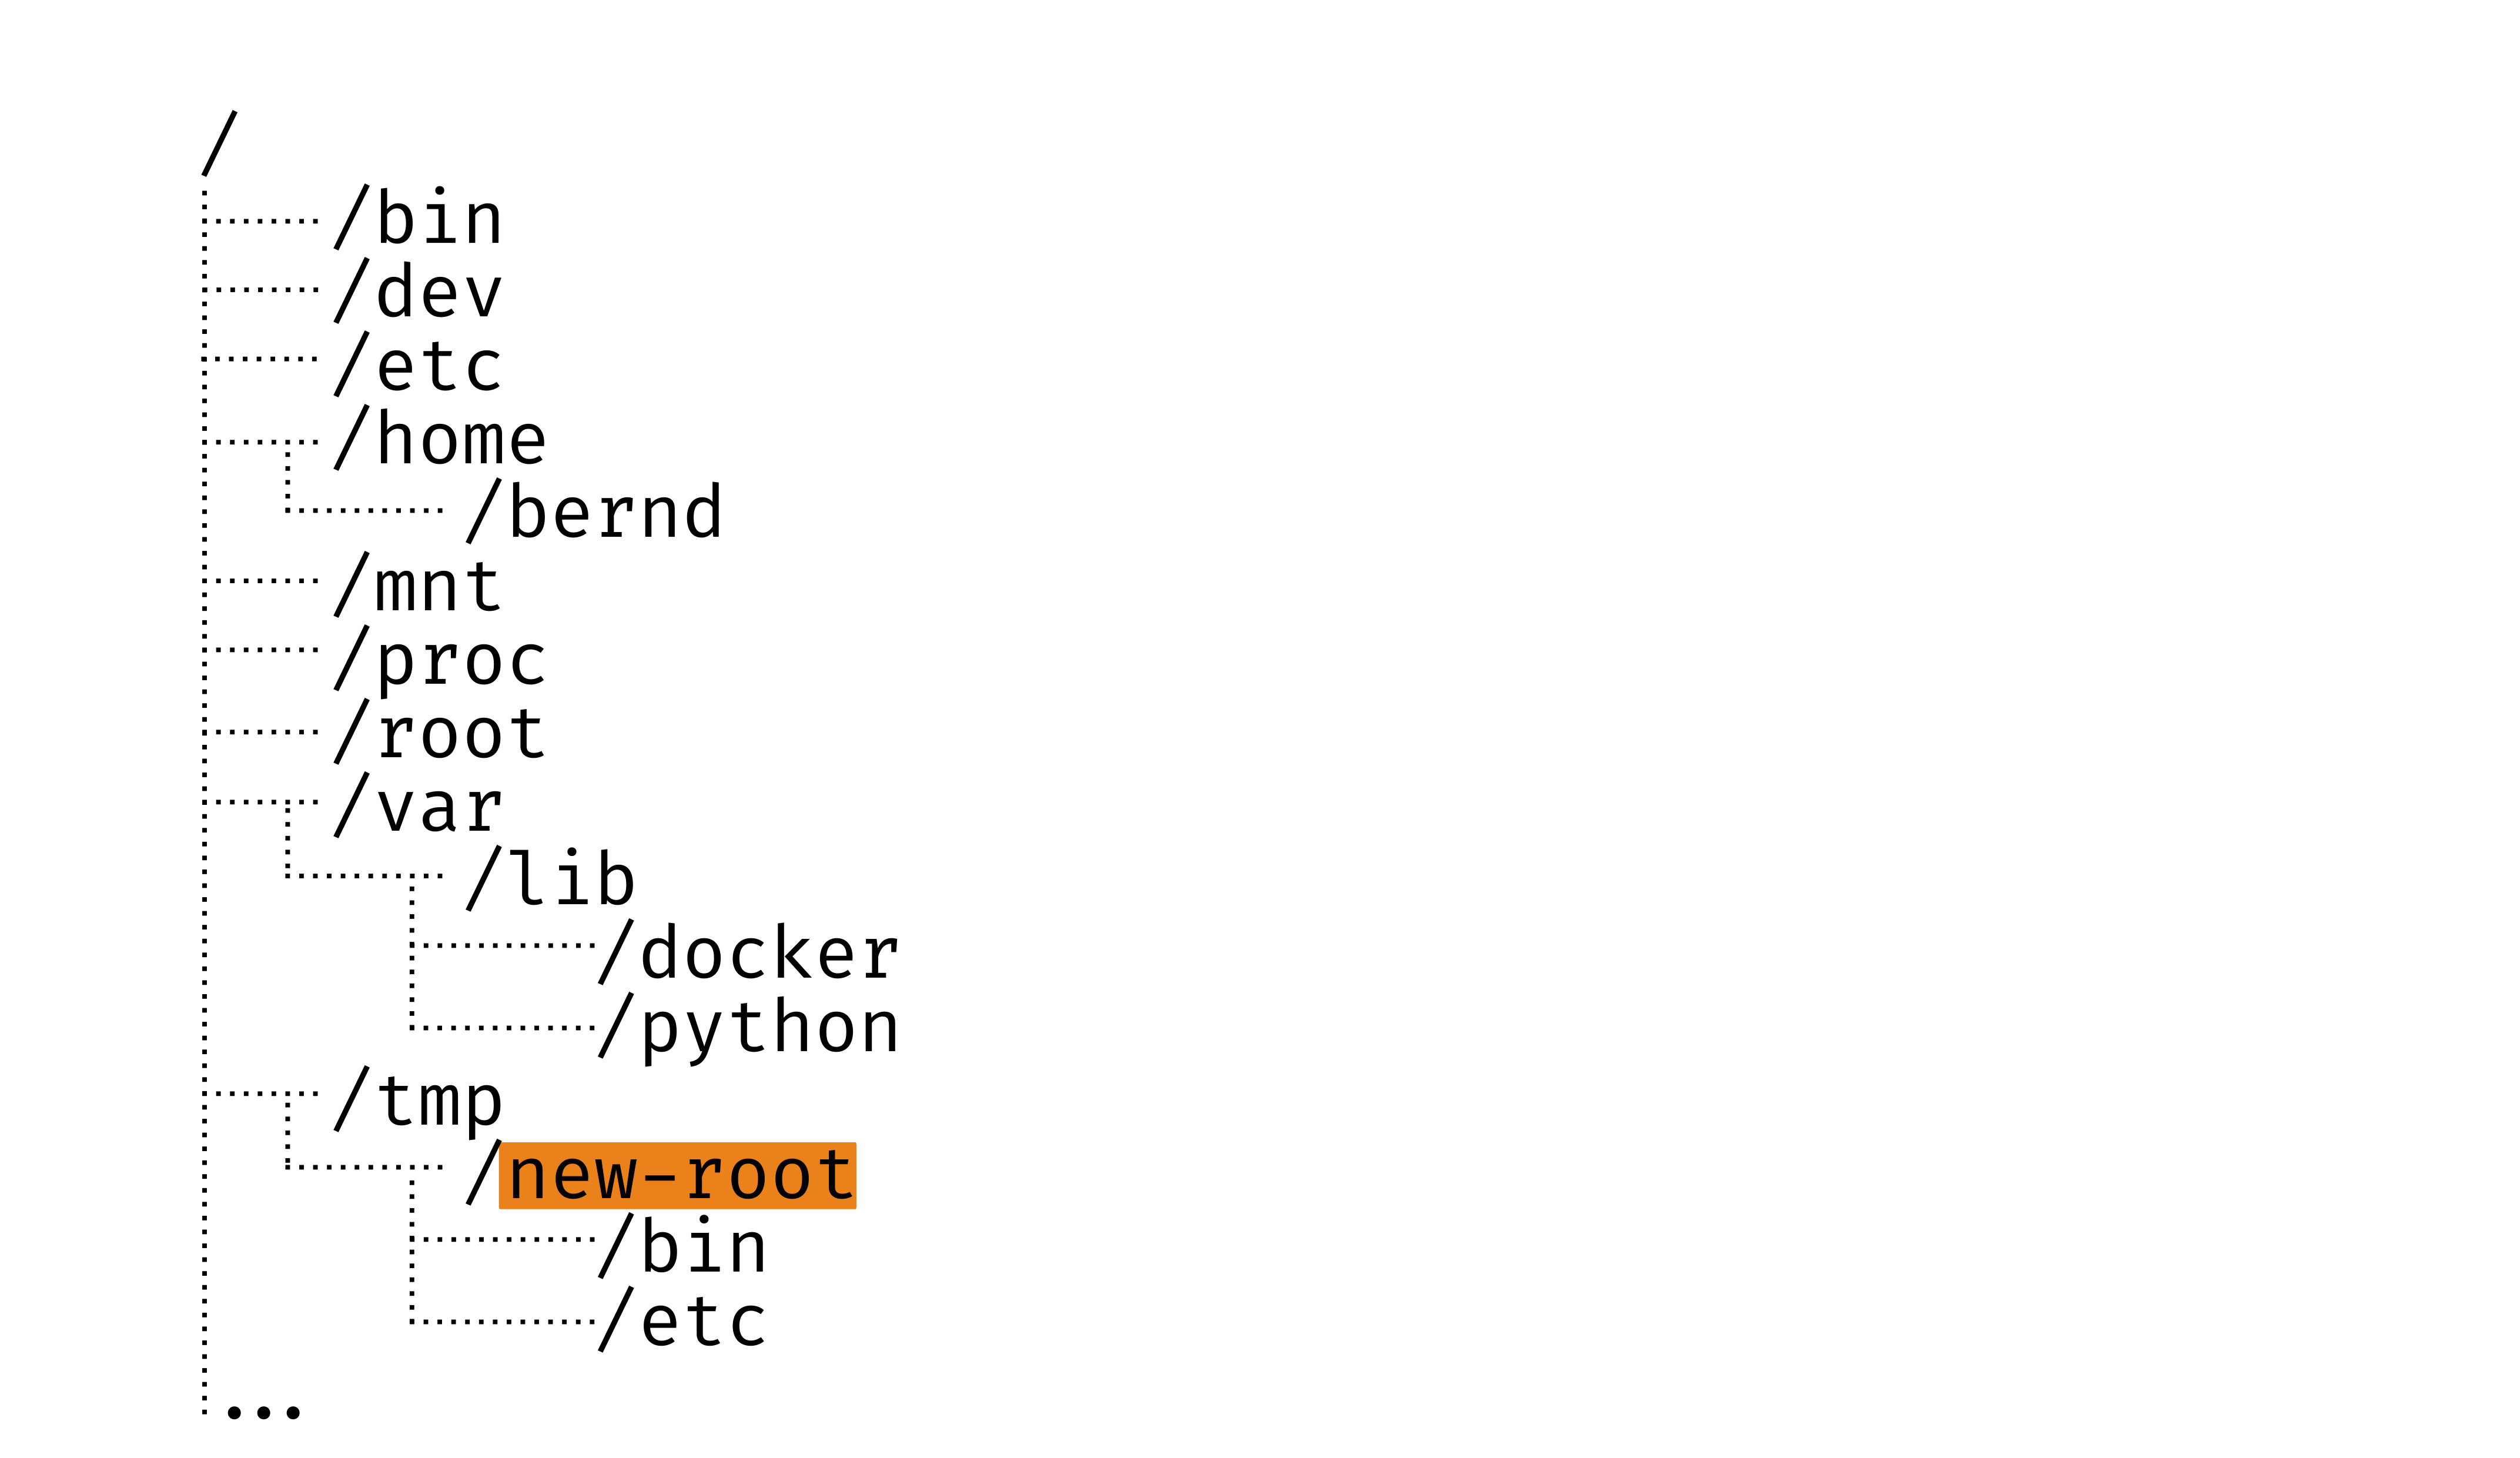
\includegraphics[width=\textwidth]{fs-tree-highlight}
  \end{frame}
  \begin{frame}[standout]
    Demo
  \end{frame}
  \begin{frame}{chroot}
    \begin{itemize}
      \item Erlaubt es das root Verzeichnis \texttt{/} neu zu setzen
      \item Sehr Hilfreich zum Debugging, compiling oder bei der Installation von Linux
      \item An sich schon sehr nützlich
      \item \textbf{Aber} noch keine Isolierung der Prozesse, User etc. von einander
    \end{itemize}
  \end{frame}
  
  \begin{frame}{Namespaces}
    \begin{itemize}[<+->]
      \item API des Linux Kernel um \textbf{virtuelle System Ressourcen} wie Netzwerk Interfaces, Mount points, UserIDs und weitere System Ressourcen zu erstellen
      \item Diese Ressourcen können einzelnen Prozessen zugewiesen
werden
      \item Können auch für sich genommen verwendet werden. Beispiel: Auf seinem eigenen Rechner mit Network-Namespaces ein Netzwerk simulieren
    \end{itemize}
  \end{frame}
  \begin{frame}[standout]
    Demo
  \end{frame}
  
  \begin{frame}{Control Groups}
    \begin{itemize}[<+->]
      \item Management von CPU Zyklen, Arbeitsspeicher oder Netzwerk Bandbreite für Gruppen von Prozessen
      \item Prozesse können in ihrem Ressourcenverbrauch eingeschränkt werden
      \item Auch seperat Nutzbar
    \end{itemize}
  \end{frame}
  \begin{frame}[standout]
    Demo
  \end{frame}

  \begin{frame}{Container}
    Container nennt man die Kombination all dieser Funktionen
  \end{frame}

  \begin{frame}{Im Alltagsgebrauch?}
    Was kann man im Alltag damit machen?
    \begin{itemize}[<+->]
      \item Wegwerf-Umgebung für Tests
      \item Isolierung einzelner Prozesse für mehr Sicherheit
      \item Netzwerktools auf eigenem PC testen
      \item CPU oder RAM hungrige Prozesse auf dem Laptop in die Schranken weisen
    \end{itemize}
  \end{frame}
  
  % % % % % %
  % Docker  %
  % % % % % %
  \section{Aber was ist jetzt Docker?}

  \begin{frame}{Docker?}
    Docker bündelt all diese Funktionen mit einfachen Werkzeugen für Entwickler
    und Sysadmins.
  \end{frame}
  \begin{frame}{Docker Images}
    \begin{itemize}[<+->]
      \item Im Prinzip Tar-Archive von Dateisystemen + Metadaten
      \item Große Auswahl an fertigen Images im Docker Hub
      \item Können einfach selbst mit sog. Dockerfiles gebaut werden
      \item Sehr portabel und erzeugen reproduziebare Ergebnisse
    \end{itemize}
  \end{frame}
  \begin{frame}{Docker Daemon}
    \begin{itemize}[<+->]
      \item Service im Hintergrund
      \item Started und managed container
      \item Baut images
      \item REST API via UNIX Socket
    \end{itemize}
  \end{frame}
  \begin{frame}{Docker CLI}
    \begin{itemize}[<+->]
      \item Interagiert mit dem Daemon
      \item Standart-Interface für Docker Entwickler und Sysadmins
      \item Werkzeug zum bauen, starten und überwachen von containern
    \end{itemize}
  \end{frame}
  \begin{frame}[standout]
    % Docker Hub -> nginx container
    % nginx container pullen und starten
    % Dockerfile anpassen, bauen starten
    % Tag und push
    Demo
  \end{frame}
  \begin{frame}{Docker Compose}
    % Beispiel compose file für die Nextcloud
    \begin{itemize}
      \item Zusätzliches Kommandozeilen Werkzeug zum Verwalten mehrer Container
      \item Konfiguration in leicht verständlichen yml Dateien
      \item Deklarativ: Beschreibung des Ergebnis, nicht der Schritte dahin
    \end{itemize}
  \end{frame}
  
  \begin{frame}{Praktische Anwendung}
    \begin{itemize}[<+->]
      \item \textbf{Konsolidierung} mehrerer Anwendungen ohne ineffiziente VMs
      \item Weg aus der \textbf{Dependency Hell}
      \item Portable \textbf{Development Environments}. Verhindert "Works on My Machine" weil alle die gleiche Version haben
      \item \textbf{Isolierung} unsicherer Prozesse von einander
      \item Ermöglicht weitreichende \textbf{Orchestrierung} auf großen Rechner-Clustern mit Failover und großer Skalierung durch Lösungen wie Kubernetes
    \end{itemize}
  \end{frame}


  % % % % % % % % %
  % Vergleich VMs %
  % % % % % % % % %
  \section{Vergleich mit VMs}

  \begin{frame}{Vergleich mit VMs}
    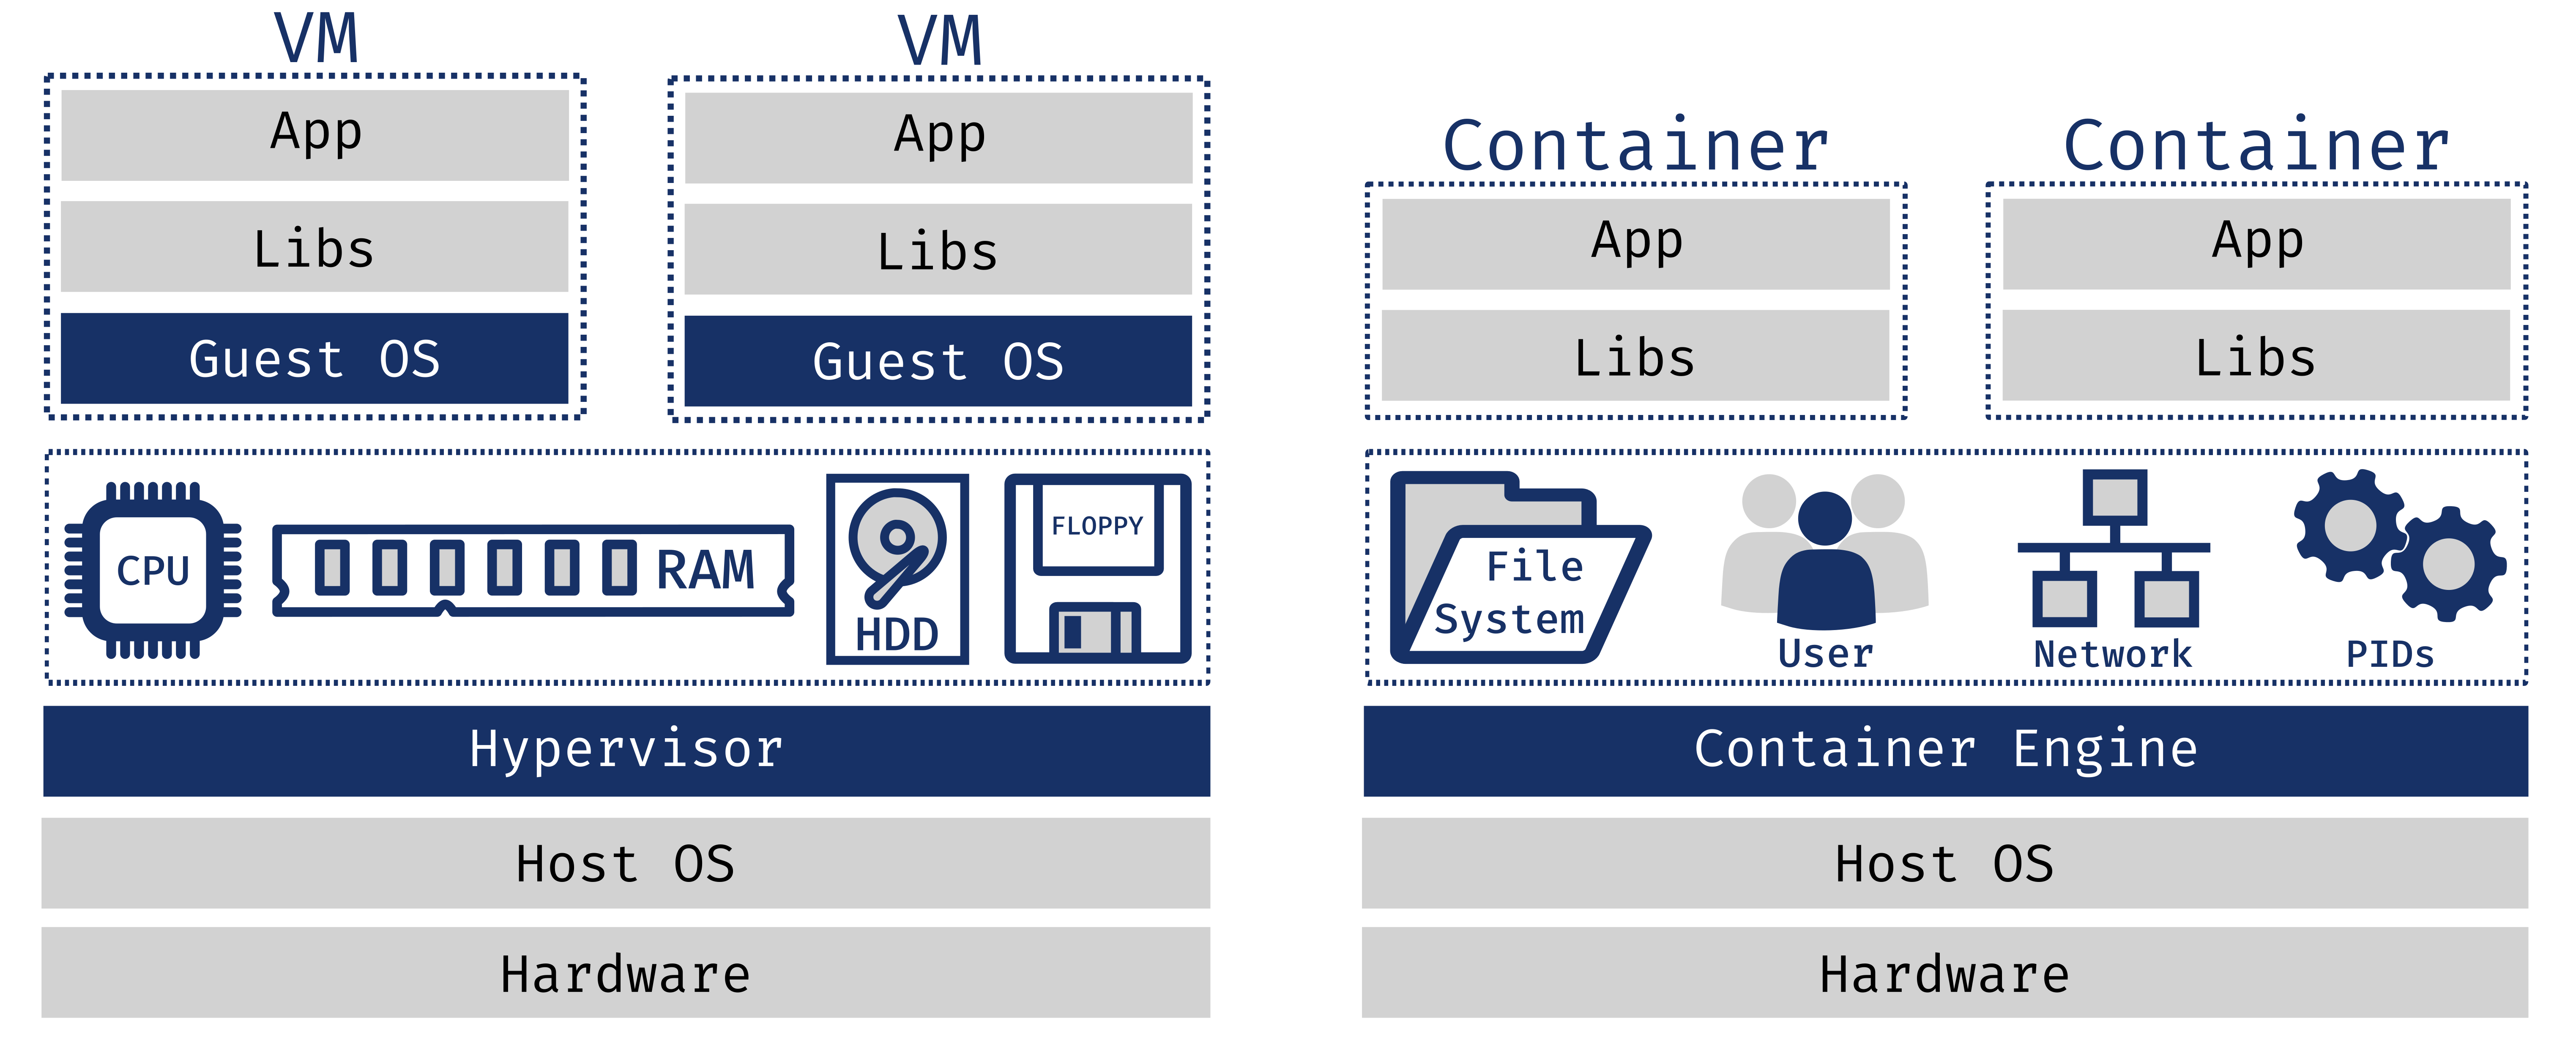
\includegraphics[width=\textwidth]{comparison}
    \textbf{Unterschied:} Bei VMs wird im Kernel/Hypervisor Hardware virtualisiert und darauf laufen andere Kernels. Container teilen sich einen Kernel, der OS-Ressourcen virtualisiert. 
  \end{frame}
  \begin{frame}{Vorteile VMs}
    \begin{itemize}
      \item Voller virtueller Computer mit allen Features
      \item Egal welcher Kernel: Linux, BSD, Windows NT, x86, x64
      \item Starke Isolierung
    \end{itemize}
  \end{frame}
  \begin{frame}{Vorteile Container}
    \begin{itemize}
      \item Effizienter: Weniger Ressourcenverbrauch und kein Boot-Vorgang
      \item Einfacher zu managen
      \item Auch einzelne Module verwendbar
      \item Alles auf einem Linux Kernel
    \end{itemize}
  \end{frame}
   
  
  % % % % % % % % % % %
  % Cioplenu Werbung  %
  % % % % % % % % % % %
  \begin{frame}[standout]
    
\includegraphics[width=0.7\linewidth]{cio-logo} \\
    cioplenu.de \\
    @AnianZ \\
    \vfill
    Wir suchen Entwickler und Sysadmins!
  \end{frame}
  \begin{frame}[standout]
    Vielen Dank! Fragen?
  \end{frame}
  
  % % % % % % % % % % % %
  % Backup: Geschichte  %
  % % % % % % % % % % % %
  \section{Container sind keine neue Erfindung}
  \begin{frame}{Geschichte}
  \begin{minipage}[c]{\linewidth}
    \color{gray}
    \only<1->{\ytl{1979}{UNIX v7: chroot system call, später in BSD}}
    \only<2->{\ytl{2000}{FreeBSD Jails}}
    \only<3->{\ytl{2001}{Linux Vserver: erste OS-Virtualisierung als Kernel Patch}}
    \only<4->{\ytl{2004}{Solaris Zones}}
    \only<5->{\ytl{2007}{Control Groups in den Linux Kernel integriert}}
    \only<6->{\ytl{2008}{LXC: Linux tooling für cgroups und namespaces}}
    \bigskip
  \end{minipage}
  \end{frame}
  \begin{frame}{Geschichte}
  \begin{minipage}[t]{\linewidth}
    \color{gray}
    \ytl{2013}{\textbf{Docker}
    \begin{itemize}
      \item Entwickler Tooling
      \item Daemon für Container Management
      \item Standartisierung
      \item Packaging in Images
      \item Docker Hub
    \end{itemize}
    --> Container werden für viele zugänglich und interessant für Entwickler}
    \end{minipage}
  \end{frame}
  \begin{frame}{Alternativen zu Docker}
    Docker ist weit nicht die einzige Container-Software auf Linux:
    \begin{itemize}
      \item LXD
      \item Rocket
      \item systemd nspawn
      \item Flatpak 
      \item Snappy
    \end{itemize}
  \end{frame}
\end{document}

